\section{Publish-subscribe systems}

Publish-subscribe is an asynchronous communication pattern where the senders of the messages or producers of the content are called \textit{publishers}, and the receivers of the messages or content consumers are called \textit {subscribers}. The subscribers express their interest in being notified and receiving content that matches their interest whenever matching contents are published \parencite{Pietzuch:2002:HDE:646854.708058}.

The two primary advantages of the publish-subscribe model are loose coupling and scalability.

\begin{itemize}
\item[]\textbf{Loose Coupling}

The publish-subscribe pattern has a widespread adoption in distributed systems due to a high degree of decoupling. This is because the publishers and subscribers have no knowledge of each other \parencite{Cheung:2010:LBC:1880018.1880020}. The co-ordination is done by an entity called the broker. Both the publishers and subscribers only communicate with the broker. The publisher publishes data without any information regarding the identity, location or the number of subscribers. Similarly, the subscribers receive the data without any information regarding the publishers. 

Unlike in traditional client-server paradigm where the client cannot send messages to the server when the server is not operational, in publish-subscribe paradigm regardless of publisher or subscriber, each can continue to operate normally. This is referred to as \textit {Time Decoupling}.   

\item[]\textbf{Scalability}

The other main advantage of this pattern is scalability. The publish-subscribe pattern provides the room for better scalability compared to traditional client-server due to message caching, parallel operation, network-based routing, etc \parencite{pub_sub_wiki}. Even outside the enterprise world publish-subscribe paradigm has proven its by providing a broad range of distributed messages via protocols such as Atom (standard) and Rich Site Summary (RSS).

\end{itemize}

In the realm of publish-subscribe the subscribers have control on what content they are interested in receiving rather than receiving all the content. This is achieved by a technique called \textit {filtering}, which also led to the different types of publish-subscribe systems \parencite{Eugster:2003:MFP:857076.857078}. We discuss two of the many types in the following sections.

\subsection{Topic-based publish-subscribe systems}

One of the popular adoptions of the publish-subscribe paradigm is the Topic-based publish-subscribe model. Although there is a subtle difference, it is also referred as subject-based or channel-based filtering. In this approach, there exists a named logical channel called \enquote{topics}. Publishers publish content/event to a given topic and subscribers interest in receiving the content/event subscribe to the topic to receive them. All the subscribers will receive the same content from a topic to which the publishers publish the content. 

It simplifies matching by having a static publisher and subscriber relationship. At the time of publication, the subscriber set is known. For a given topic, every content/event published on a topic is received by the same subscriber set unless topics or subscriptions change. Figure \ref{figures:topic_pub_sub} depicts a topic-based publish-subscribe model.

    \makeatletter
    \setlength{\intextsep}{20pt}
    \makeatother

    \begin{figure}[h!]
    \centering
    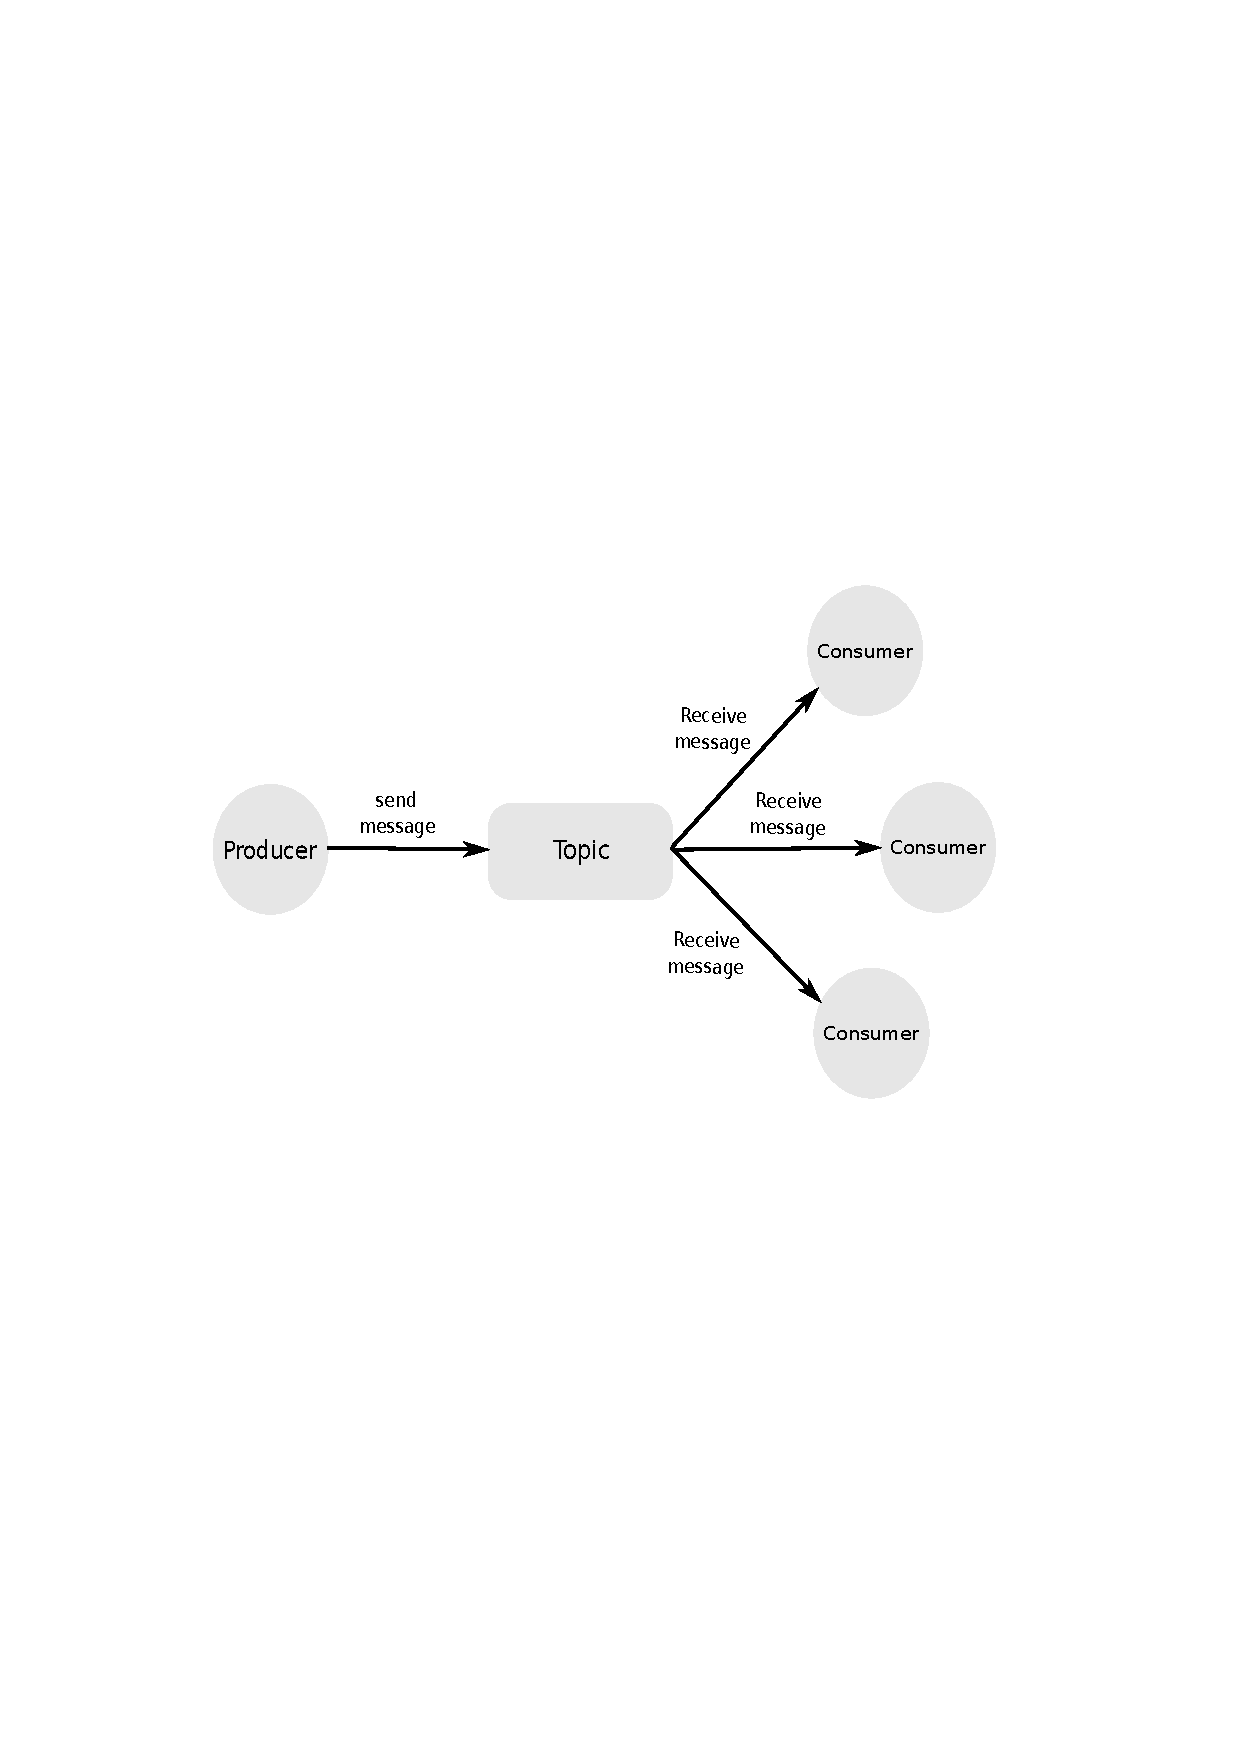
\includegraphics[width=.9\textwidth, trim={0 10cm 0 9cm},clip]{topic_pub_sub.pdf}
    \caption{Topic-based publish-subscribe}\label{figures:topic_pub_sub}
    \end{figure}

Topics are hierarchically organized. Subscriptions can contain wildcards to match multiple topics; however, the publisher cannot use wildcards within a topic to publish event/content.

\begin{itemize}
\item[]\textbf{Hierarchically organized topics}
    \begin{itemize}
    \item E.g., news/sports/cricket
    \item E.g., news/sports/football
    \end{itemize}

\item[]\textbf{Topic subscription using wildcard}
    \begin{itemize}
    \item E.g., news/sports/*
    \end{itemize}
\end{itemize}



\subsection{Content-based publish-subscribe systems}

Content-based publish-subscribe system provides more flexibility \parencite{Aguilera:1999:MEC:301308.301326} and expressiveness to subscriber in expressing interest \parencite{Shen2010}. It provides a query based approach to come filters over the content by using a \textit {subscription language}. Thus provides more precise matching of interest. Figure \ref{figures:content_pub_sub} shows an example of a content-based publish-subscribe system.

    \makeatletter
    \setlength{\intextsep}{20pt}
    \makeatother

    \begin{figure}[h!]
    \centering
    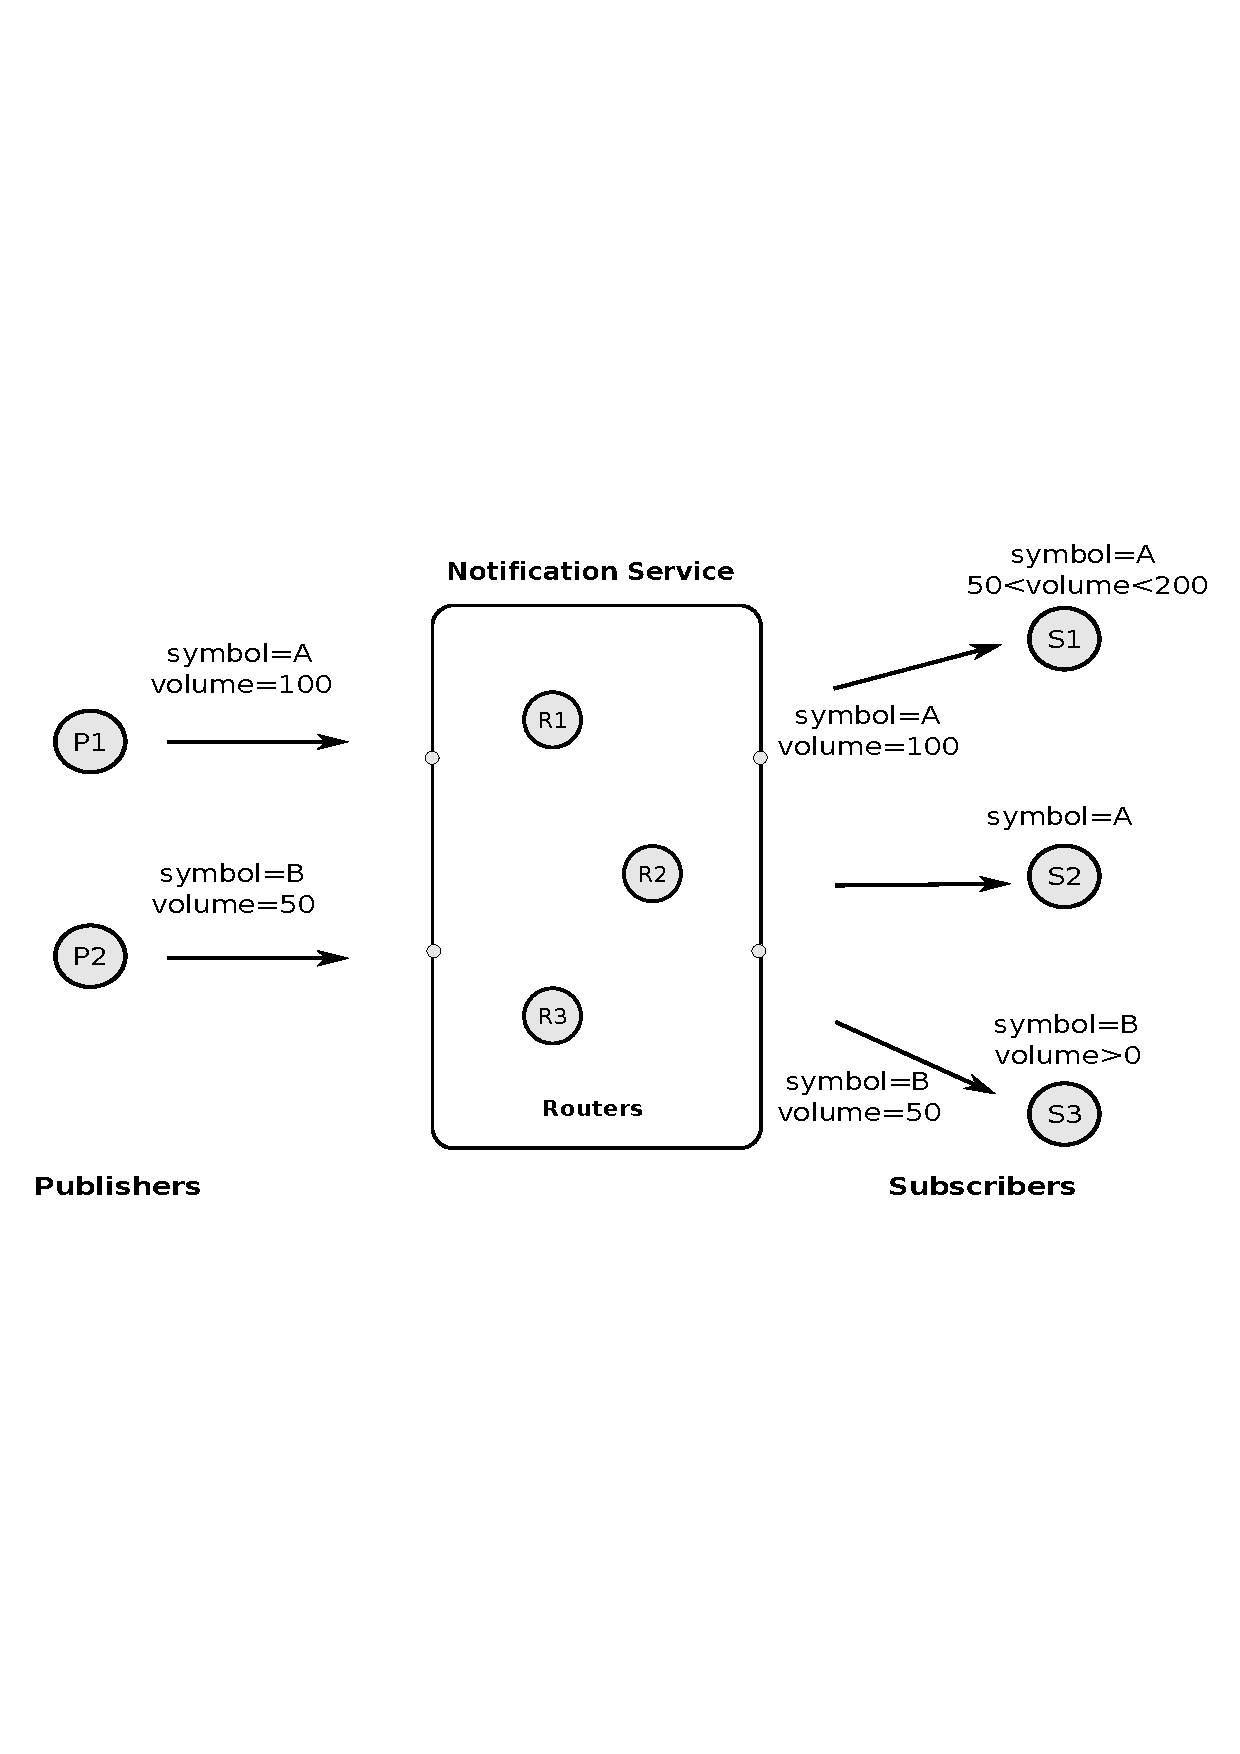
\includegraphics[keepaspectratio, width=.8\textwidth, trim={0 8cm 0 8cm},clip]{content_pub_sub.pdf}
    \caption{Content-based publish-subscribe}\label{figures:content_pub_sub}
    \end{figure}

Unlike topic-based model, here the notifications of events are grouped based on the runtime query calculations rather than predefined constraints. This provides high flexibility and more expressiveness, but these advantages also comes at a cost. Since the event/content receivers are not known previously, the interested subscribers are determined at runtime requiring more resources.  

